\documentclass{article}


\usepackage{PRIMEarxiv}

\usepackage[utf8]{inputenc} % allow utf-8 input
\usepackage[T1]{fontenc}    % use 8-bit T1 fonts
\usepackage{hyperref}       % hyperlinks
\usepackage{url}            % simple URL typesetting
\usepackage{booktabs}       % professional-quality tables
\usepackage{amsfonts}       % blackboard math symbols
\usepackage{nicefrac}       % compact symbols for 1/2, etc.
\usepackage{microtype}      % microtypography
\usepackage{lipsum}
\usepackage{graphicx}
\usepackage{booktabs, multirow} 
\usepackage{caption}
\usepackage{subcaption}
\usepackage{tikz}
\usepackage{pgfplots}
\usepackage{amsmath,amssymb}
\usepackage{todonotes}
\usepackage{caption} 
\captionsetup[table]{skip=10pt}
\DeclareMathOperator{\E}{\mathbb{E}}
\graphicspath{{media/}}     % organize your images and other figures under media/ folder


%% Title
\title{We Didn't Start The Fire: Robust Wildfire Detection With Limited Labeled Data}

\author{
  Ivanina Ivanova, Abhay Mathur \\
  Institut Polytechnique de Paris \\
  \texttt{\{abhay.mathur, ivanina.ivanova\}@ip-paris.fr} \\
  %% examples of more authors
}


\begin{document}
\maketitle

\begin{abstract}
\end{abstract}

\section{Problem Statement}
This project aims to develop a fire detection system using a designated
dataset. The dataset consists of three subsets: a training set, a validation
set, and a test set. Specific constraints and guidelines must be strictly
followed to ensure compliance with the project requirements.

\subsection{Dataset Access and Constraints}

The dataset is available for download from Kaggle~\footnote{Wildfire Dataset:
  \url{https://www.kaggle.com/datasets/abdelghaniaaba/wildfire-prediction-dataset/code}}.
% \url{https://www.kaggle.com/datasets/abdelghaniaaba/wildfire-prediction-dataset/code}.
It comprises a training set, a validation set, and a test set. A critical
restriction is imposed on the training set: its labels are inaccessible. Any
direct utilization of annotations from the training set will lead to
disqualification.

\subsection{Dataset Partitioning}

To facilitate model training, the original validation set must be partitioned
into a newly defined validation set and a new training set. The original
training set may be leveraged in a creative manner; however, its labels must
not be employed under any circumstances.

\subsection{Model Development}

A deep neural network (DNN) will be trained utilizing the newly defined
training and validation sets. Various methodologies and supplementary resources
may be incorporated to enhance model performance, provided that all constraints
related to annotation usage are rigorously upheld.

\section{Dataset Analysis}

The dataset consists of satellite images of areas that previously experienced
wildfires in Canada. According to the problem statement, we discard the labels
of the training set and split the validation dataset into labeled training and
validation sets in a 4:1 ratio. The resulting splits are as follows:

\begin{itemize}
  \item Train: 5040 images
  \item Train unlabeled: 30249 images
  \item Val: 1260 images
  \item Test: 6299 images
\end{itemize}

We show some representative images from the dataset in
Figure~\ref{fig:samples}. A visual inspection of the dataset showed that most
wildfire images contain more vegetation, while non-wildfire images pertain to
urban locations.

\begin{figure}
  \centering
  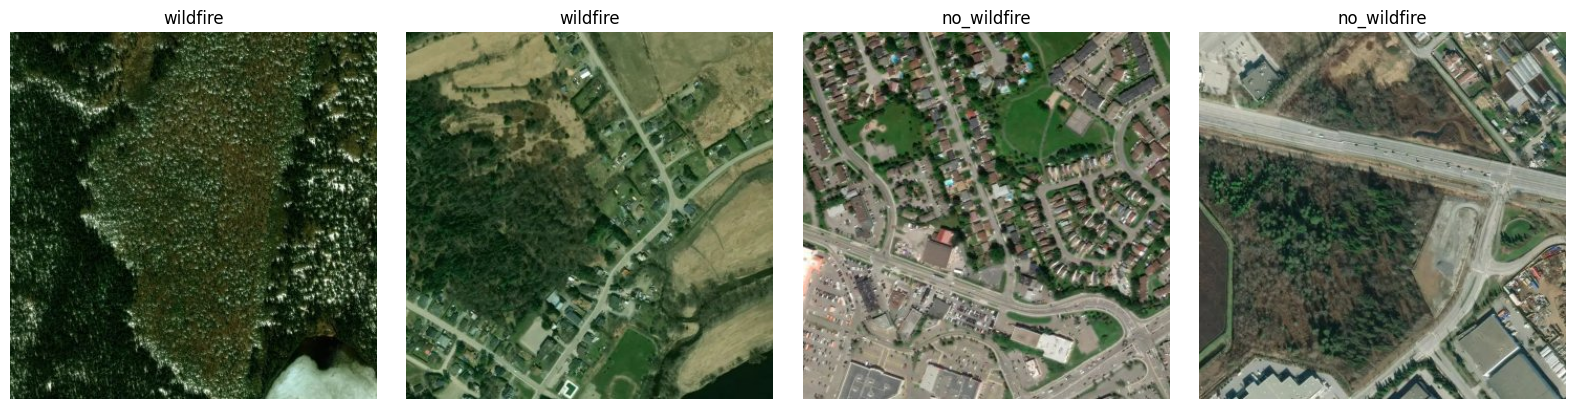
\includegraphics[width=0.8\textwidth]{figures/samples2.png}
  \caption{Some sample images from the dataset.}
  \label{fig:samples}
\end{figure}

The coordinates of the location of the images can be extracted from the
filename. We show the spread of images with respect to labels in
Figure~\ref{fig:coordinate_analysis}. This shows that there are some clusters
consistent across splits where wildfires can be expected.

\begin{figure}
  \centering
  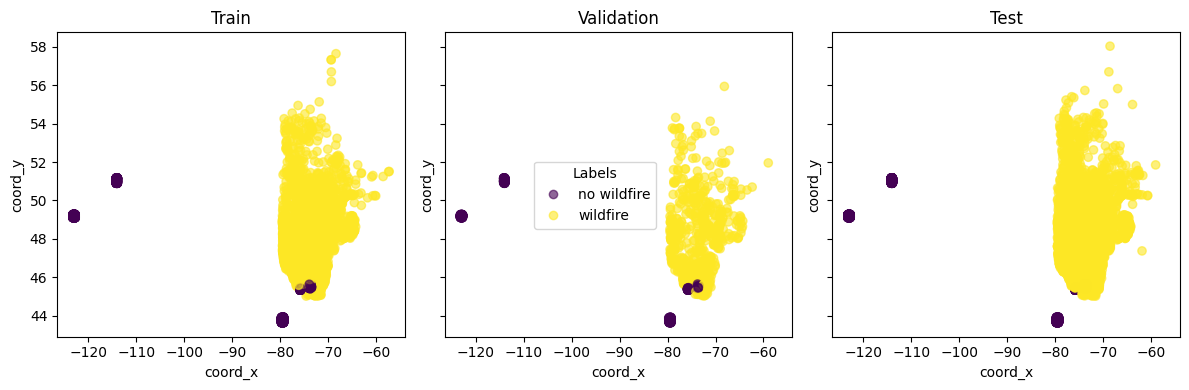
\includegraphics[width=0.8\textwidth]{figures/coord_label.png}
  \caption{Spatial Distribution of the Dataset. All splits show a similar spread of zones where fires occured.}
  \label{fig:coordinate_analysis}
\end{figure}

\section{Baselines: Using Available Labeled Data}

\subsubsection{Naive Coordinates Classifier}
A simple baseline that assigns labels based solely on coordinate information.
This approach assumes that spatial location alone is a strong enough feature
for classification.

\subsubsection{Image Classifiers}
We train a series of image classifiers using Convolutional Neural Networks
(CNNs) to classify images based on their visual content. We experiment with
different CNN architectures, including ResNet18, ResNet34, ResNet50, and
ResNet101.

\subsubsection{Fused Classifiers}
We combine the coordinate-based classifier with the image classifiers to create
a fused model that leverages both spatial and visual features for
classification.

\section{Learning from Unlabeled Data}

In this section, we discuss our methods for learning from unlabeled data. We
explore various self-supervised learning techniques to extract useful
representations from the dataset. These representations are then used to train
a classifier on the labeled data.

\subsection{SimCLR}
SimCLR~\cite{simclr} is a self-supervised learning method that learns visual
representations by maximizing the agreement between differently augmented views
of the same data example.

The training pipeline of SimCLR consists of the following steps:

\begin{figure}[!t]
  \small
  \centering
  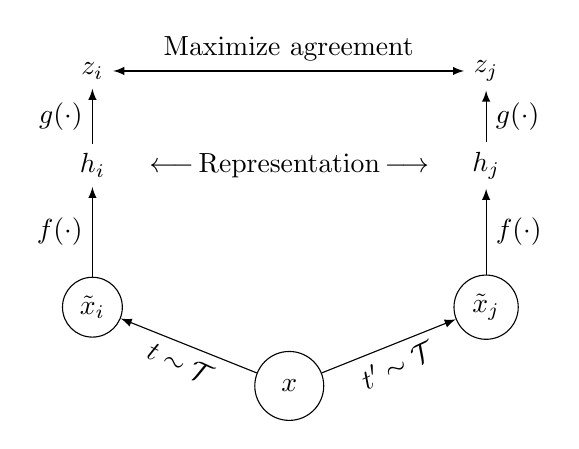
\begin{tikzpicture}
    \node at (0,1.8) (h) {$\longleftarrow\,$Representation$\,\longrightarrow$};
    \node[draw, circle] at (0,-1) (x) {$\,~{x}~\,$};
    \node[draw, circle] at (-2.5,0) (x1) {$\tilde{{x}}_i$};
    \node[draw, circle] at (2.5,0) (x2) {$\tilde{{x}}_j$};
    \node at (-2.5,1.8) (h) {$ h_i$};
    \node at (2.5,1.8) (c) {$ h_j$};
    \node at (-2.5,3) (hh) {$ z_i$};
    \node at (2.5,3) (cc) {$ z_j$};
    \path[->]
    (x)  edge [>=latex] node[below,rotate=-25] {$t\sim\mathcal{T}$} (x1)
    (x)  edge [>=latex] node[below,rotate=25] {$t'\sim \mathcal{T}$} (x2)
    (x1)  edge [>=latex] node[left,rotate=0] {$f(\cdot)$} (h)
    (x2)  edge [>=latex] node[right,rotate=0] {$f(\cdot)$} (c)
    (h)  edge [>=latex] node[left,rotate=0] {$g(\cdot)$} (hh)
    (c)  edge [>=latex] node[right,rotate=0] {$g(\cdot)$} (cc);
    \path[<->]
    (hh)  edge [>=latex] node[above,rotate=0] {Maximize agreement} (cc);
  \end{tikzpicture}
  \caption{Framework for SimCLR~\cite{simclr}.
    Two separate data augmentation operators are sampled and applied to each data example to obtain two correlated views.
    A base encoder network $f(\cdot)$ and a projection head $g(\cdot)$ are trained to maximize agreement using a contrastive loss.
    After training is completed, we simply use the encoder $f(\cdot)$ and representation $ h$ for downstream tasks.}\label{fig:framework}
\end{figure}

\subsubsection{Data Augmentation}
Each input image is transformed into two different augmented views through a
series of random augmentations such as cropping, resizing, flipping, color
jittering, and Gaussian blurring. These augmentations are crucial as they
create diverse views of the same image, which the model learns to recognize as
similar.

\subsubsection{Encoder Network and Projection Head}
Both augmented views are passed through an encoder network (typically a ResNet)
to obtain their respective feature representations. The encoder network is
shared between the two views.

The feature representations are then passed through a small neural network
called the projection head, which maps them to a latent space where the
contrastive loss is applied. The projection head typically consists of a few
fully connected layers.

\subsubsection{Contrastive Loss}
The core idea of SimCLR is to bring the representations of the two augmented
views of the same image closer together in the latent space while pushing apart
representations of different images. This is achieved using a contrastive loss
function, specifically the normalized temperature-scaled cross-entropy loss
(NT-Xent loss). The loss function is defined as:

\begin{align}
  \mathcal{L}_{i,j} & = -\log
  \frac{\exp(\text{sim}(\mathbf{z}_i, \mathbf{z}_j) / \tau)}{\sum_{k=1}^{2N}
  \mathbb{1}_{[k \neq i]} \exp(\text{sim}(\mathbf{z}_i, \mathbf{z}_k) / \tau)}
  \label{eq:simclr}
\end{align}

Where $\mathbf{z}_i$ and $\mathbf{z}_j$ are the latent representations of the
two augmented views of the same image, $\text{sim}(\cdot, \cdot)$ denotes the
cosine similarity, $\tau$ is a temperature parameter, and $N$ is the batch
size.

\subsection{Variational Autoencoder (VAE)}

\subsubsection{$\beta$-VAE}
A Variational Autoencoder (VAE) was used as a self-supervised learning approach
to extract latent representations from the training dataset. The VAE comprises
an encoder network, which maps input images to a latent space distribution, and
a decoder network, which reconstructs the input from latent variables. The
encoder network consists of a series of convolutional layers followed by fully
connected layers, while the decoder network mirrors the encoder architecture.
The VAE was trained using the unlabeled training dataset. The training
objective that we decided to use is Beta-VAE~\cite{beta-vae}. Beta-VAE is a
modification of the original VAE that introduces a hyperparameter $\beta$ to
the loss function. The $\beta$ parameter controls the trade-off between the
reconstruction loss and the Kullback-Leibler divergence. The loss function for
the Beta-VAE is given by:

\begin{align}
  \mathcal{L}(\theta, \phi, x, z, \beta) & = \E_{q_\phi(z|x)}[\log p_\theta(x|z)] - \beta D_{KL}(q_\phi(z|x)\| p(z))
\end{align}

where $p(z|x)$ is the learned posterior, $p(z)$ is the prior distribution
(assumed to be Gaussian), and $p(x|z$) represents the likelihood of
reconstructing the input image from the latent space. Well chosen $\beta$
values can lead to disentangled representations in the latent space. The VAE
was trained for 50 epochs using the Adam optimizer with a learning rate of
0.0001.
\\\
\\\
\textbf{Latent Representation Classifier}
The latent representations obtained from the VAE were then used to
train a classifier. The classifier consists of a two fully connected layer with
a ReLU activation fucntion and a Dropout of 0.2 layer in between. The classifier was
trained using the labeled train dataset. The training objective was to minimize
the binary cross-entropy loss between the predicted and true labels. The linear
classifier was trained for 20 epochs using the Adam optimizer with a learning
rate of 0.0001.

\subsubsection{ResNet-based Encoder}
To further improve the quality of the learned latent representations, we experimented with a ResNet-based encoder. The idea is to replace the standard convolutional layers with a ResNet architecture, this modification will help in capturing richer hierarchical features and improved the overall reconstruction quality, leading to better downstream classification performance.

\subsubsection{Vector Quantized Variational Autoencoder (VQ-VAE)}
Additionally, we experimented with a Vector Quantized Variational Autoencoder (VQ-VAE)~\cite{vq-vae}. The difference between VQ-VAE and the standard VAE is that VQ-VAE is using a discrete latent space instead of a continuous one. Instead of learning a probabilistic distribution in the latent space, VQ-VAE learns a set of discrete latent embeddings. The encoding process involves mapping an input image to the closest embedding vector from a learned codebook, effectively quantizing the latent representations. The loss function for VQ-VAE consists of three terms:

\begin{align}
  \mathcal{L}(x, z) & = \log p(x|z_q(x)) + | sg[z_e(x)] - e |_2^2 + \beta | z_e(x) - sg[e]  |_2^2
\end{align}



where $z_e$ is the encoder output, $z_q$ is the nearest codebook entry, and $sg[\cdot]$ is the stop-gradient operator. The first term represents the reconstruction loss, the second term ensures the encoder output stays close to the codebook entries, and the third term encourages the codebook entries to move toward the encoder outputs. The advantage of VQ-VAE is that it prevents posterior collapse, a common issue in VAEs where the latent representations become overly dependent on the prior, leading to poor representation learning. By enforcing a discrete latent space, VQ-VAE learns more interpretable and structured representations, which significantly improved the downstream classification task.
\\\
\\\
\textbf{ResNet VQ-VAE}
Same as the VAE we implemented a ResNet-based encoder for the VQ-VAE (ResNet VQ-VAE). The combination of ResNet and VQ-VAE provided both robust feature extraction and structured latent representations, leading to improved performance in our classification task. We used the same classifier architecture as in the VAE experiments.

Our results demonstrate that moving from a standard VAE to a ResNet-based encoder and finally to VQ-VAE with ResNet led to progressively better latent representations and improved classification performance.


\subsection{Pseudo-Labeling}

Pseudo-labeling is a semi-supervised learning technique that leverages
unlabeled data to improve model performance. The approach involves training an
initial model on labeled data and then using its predictions on unlabeled
samples as pseudo-labels. These pseudo-labeled samples are subsequently
incorporated into the training process alongside the original labeled data,
effectively increasing the dataset size and improving generalization.

In our experiments, we applied pseudo-labeling from larger models to simpler
CNN-based architectures to assess its impact on classification performance.

\section{Experiments and Results}

\subsection{Experimental Setup}

To evaluate the effectiveness of different classification approaches, we
conducted a series of experiments comparing models with and without
pre-training. Our experiments were designed to assess the impact of feature
extraction, coordinate-based classification, and various pre-training
strategies on classification performance.

We first established baseline models using a simple Coordinate Classifier, a
standard CNN, and a combined CNN + Coordinate Classifier. These models allowed
us to determine the effectiveness of coordinate information in enhancing
classification accuracy.

The Coordinate Classifier is an MLP with one hidden layer with 64 units and a
ReLU activation function. The CNN model consists of four convolutional layers
followed by two fully connected layers with ReLU activation functions. The CNN
+ Coordinate Classifier combines the CNN model with the Coordinate Classifier
to leverage both feature-based and coordinate-based classification.

Next, we evaluated feature-based classifiers using different ResNet
architectures (ResNet18, ResNet34, ResNet50, and ResNet101). We further
extended this analysis by incorporating coordinate information alongside
feature-based classification, measuring the improvements in accuracy and
F1-score across varying model complexities.

To examine the impact of pre-training, we tested models trained with
self-supervised and semi-supervised learning techniques, including SimCLR and
pseudo-labeling. The SimCLR pre-training was applied to ResNet architectures to
assess the benefits of contrastive learning. Results from the pre-training can
be found in Table~\ref{tab:simclr}.

\begin{table}[!htp]\centering
  \caption{Results of Pre-Training with SimCLR. The reconstructin loss is the one defined in Eq~\ref{eq:simclr}}\label{tab:simclr}
  \scriptsize
  \begin{tabular}{lrr}\toprule
    \textbf{Backbone} & \textbf{\#params} & \textbf{Reconstruction Loss} \\\midrule
    ResNet18          & 11.50M            & 0.164                        \\
    ResNet34          & 21.61M            & 0.158                        \\
    ResNet50          & 27.97M            & 0.162                        \\
    ResNet101         & 46.96M            & 0.182                        \\
    \bottomrule
  \end{tabular}
\end{table}

We use the best model from the previous experiments (Feature + Coordinate
classifier with ResNet34 backbone without pre-training) to generate
pseudo-labels on the unlabeled training set. We then train a CNN model and a
Coordinates+CNN model with an aggregation of the pseudo-labeled and the
labelled set and evaluate their performance on the test set.

Additionally, we explored latent representation learning methods by training
classifiers using $\beta$-VAE and VQ-VAE. These experiments aimed to determine
whether unsupervised representation learning could provide a competitive
alternative to direct feature extraction from supervised learning.

For all experiments, we record classification accuracy and F1-score as primary
evaluation metrics. All experiments were conducted on a single NVIDIA A100 GPU
with 40GB vRAM.

\subsection{Results}

\begin{table}[!htp]\centering

  \caption{Performance comparison of various models with and without pre-training.}\label{tab:global_results}
  \scriptsize
  \begin{tabular}{cllccc}\toprule
    \textbf{Pre-Training}             & \textbf{Model}                                   & \textbf{Backbone} & \textbf{\#params} & \textbf{Accuracy} & \textbf{F1 Score} \\ \cmidrule{1-6}
    ---                               & Coordinate Classifier                            & ---               & \textbf{4.417K}   & 0.855             & 0.873             \\ \cmidrule{1-6}
    ---                               & CNN                                              & ---               & 14.912M           & 0.9446            & 0.9491            \\ \cmidrule{1-6}
    ---                               & CNN + Coordinate Classifier                      & ---               & 14.913M           & 0.9832            & 0.9849            \\ \cmidrule{1-6}
    \multirow{4}{*}{---}              & \multirow{4}{*}{Feature Classifier}              & ResNet18          & 11.441M           & 0.983             & 0.984             \\
                                      &                                                  & ResNet34          & 21.549M           & 0.98              & 0.982             \\
                                      &                                                  & ResNet50          & 27.711M           & 0.985             & 0.986             \\
                                      &                                                  & ResNet101         & 46.703M           & 0.978             & 0.98              \\ \cmidrule{1-6}
    \multirow{4}{*}{---}              & \multirow{4}{*}{Feature + Coordinate Classifier} & ResNet18          & 11.442M           & 0.9916            & 0.9924            \\
                                      &                                                  & ResNet34          & 21.550M           & \textbf{0.9921}   & \textbf{0.9928}   \\
                                      &                                                  & ResNet50          & 24.560M           & 0.9906            & 0.9915            \\
                                      &                                                  & ResNet101         & 43.552M           & 0.99              & 0.991             \\ \cmidrule{1-6}
    \multirow{4}{*}{SimCLR}           & \multirow{4}{*}{Feature Classifier}              & ResNet18          & 11.523M           & 0.98              & 0.982             \\
                                      &                                                  & ResNet34          & 21.631M           & 0.976             & 0.978             \\
                                      &                                                  & ResNet50          & 27.988M           & 0.984             & 0.985             \\
                                      &                                                  & ResNet101         & 46.980M           & 0.984             & 0.985             \\ \cmidrule{1-6}
    \multirow{2}{*}{Pseudo Labelling} & CNN                                              & ---               & 14.912M           & 0.971             & 0.9737            \\
                                      & CNN+Coordinate Classifier                        & ---               & 14.913M           & 0.9867            & 0.9879            \\\cmidrule{1-6}
    \multirow{6}{*}{$\beta$-VAE}      & Feature Classifier                               & -                 & 72.21K            & 0.887             & 0.9               \\\cmidrule{2-6}
                                      & \multirow{5}{*}{Feature + Coordinate Classifier} & -                 & 73.43K            & 0.936             & 0.943             \\
                                      &                                                  & ResNet18          & 27.83K            & 0.934             & 0.942             \\
                                      &                                                  & ResNet34          & 48.04K            & 0.926             & 0.935             \\
                                      &                                                  & ResNet50          & 55.64K            & 0.915             & 0.926             \\
                                      &                                                  & ResNet101         & 93.62K            & 0.944             & 0.950             \\\cmidrule{1-6}
    \multirow{5}{*}{VQ-VAE}           & Feature Classifier                               & -                 & 96.64K            & 0.931             & 0.936             \\ \cmidrule{2-6}
                                      & \multirow{4}{*}{Feature + Coordinate Classifier} & ResNet18          & 46.29K            & 0.906             & 0.920             \\
                                      &                                                  & ResNet34          & 66.51K            & -                 & -                 \\
                                      &                                                  & ResNet50          & 70.96K            & 0.959             & 0.968             \\
                                      &                                                  & ResNet101         & 108.9K            & -                 & -                 \\\midrule
    \bottomrule
  \end{tabular}
\end{table}

We present our final results in Table~\ref{tab:global_results}. These results
demonstrate the impact of model architecture, coordinate information, and
pre-training strategies on classification performance, as measured by accuracy
and F1-score.

The baseline models without pre-training reveal significant differences in
performance. The Coordinate Classifier alone achieves an accuracy of 85.5\%,
which is considerably lower than other methods, highlighting its limited
capacity to classify effectively based solely on coordinate information. In
contrast, the standard CNN model without coordinate features attains a much
higher accuracy of 94.46\%. Notably, the combination of CNN and Coordinate
Classifier further improves accuracy to 98.32\%, demonstrating that
incorporating coordinate features enhances classification performance.

Feature-based models utilizing ResNet backbones show consistently strong
performance. Among them, ResNet50 achieves an accuracy of 98.5\%, outperforming
both ResNet18 and ResNet34. However, ResNet101 exhibits a slight drop in
accuracy to 97.8\%, suggesting potential overfitting or optimization challenges
with deeper networks. When coordinate information is incorporated alongside
feature-based classification, performance improves across all ResNet
architectures. The best-performing model in this category is the Feature +
Coordinate Classifier with ResNet34, which attains the highest accuracy of
99.21\% and an F1-score of 99.28\%, outperforming deeper ResNet variants. This
suggests that ResNet34 provides an optimal balance of depth and generalization
in this setting.

Pre-training strategies yield mixed results. SimCLR, a self-supervised
contrastive learning approach, demonstrates potential benefits, but results for ResNet50,  achieves an accuracy of 98.2\%. While
competitive, this performance does not surpass the best fully supervised
models. Pseudo-labeling improves performance for CNN-based models, raising the
accuracy of a standard CNN to 97.1\% and CNN + Coordinate Classifier to
98.67\%, indicating that leveraging unlabeled data can enhance classification
but does not surpass the best fully supervised methods.

Latent representation learning methods such as $\beta$-VAE and VQ-VAE show
comparatively lower performance. The best-performing $\beta$-VAE model with
ResNet101 and coordinate information achieves 94.4\% accuracy, while VQ-VAE with
ResNet50 and coordinate information attains 95.9\%. These results suggest that
while variational autoencoders can learn meaningful representations, they do
not outperform direct supervised learning approaches.

Overall, the highest accuracy is achieved by the Feature + Coordinate
Classifier using a ResNet34 backbone, indicating that incorporating coordinate
information alongside feature extraction is crucial for maximizing
classification performance. Furthermore, while pre-training methods contribute
to performance improvements, they do not surpass the best purely supervised
models, suggesting that direct supervised learning remains the most effective
strategy for this classification task.

\subsection{Error Analysis}

While our best model has an accuracy of more than 99\%, it is essential to
understand the errors made by the model. We analyze the confusion matrix of the
best model and visualise the samples that were misclassified in
Figure~\ref{fig:error_analysis}.

\begin{figure}[!t]
  \centering
  \begin{subfigure}{0.325\textwidth}
    \centering
    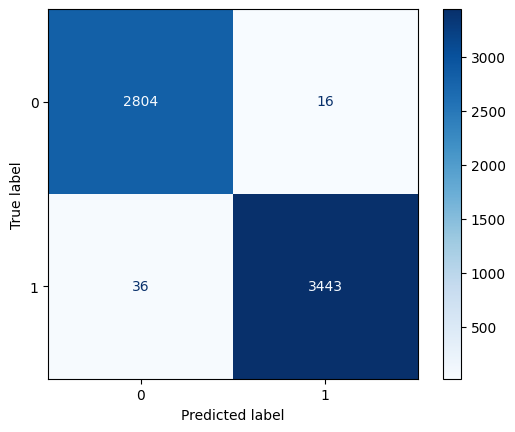
\includegraphics[width=\textwidth]{figures/confusion.png}
    \caption{Confusion Matrix}
  \end{subfigure}%
  \hfill
  \begin{subfigure}{0.65\textwidth}
    \centering
    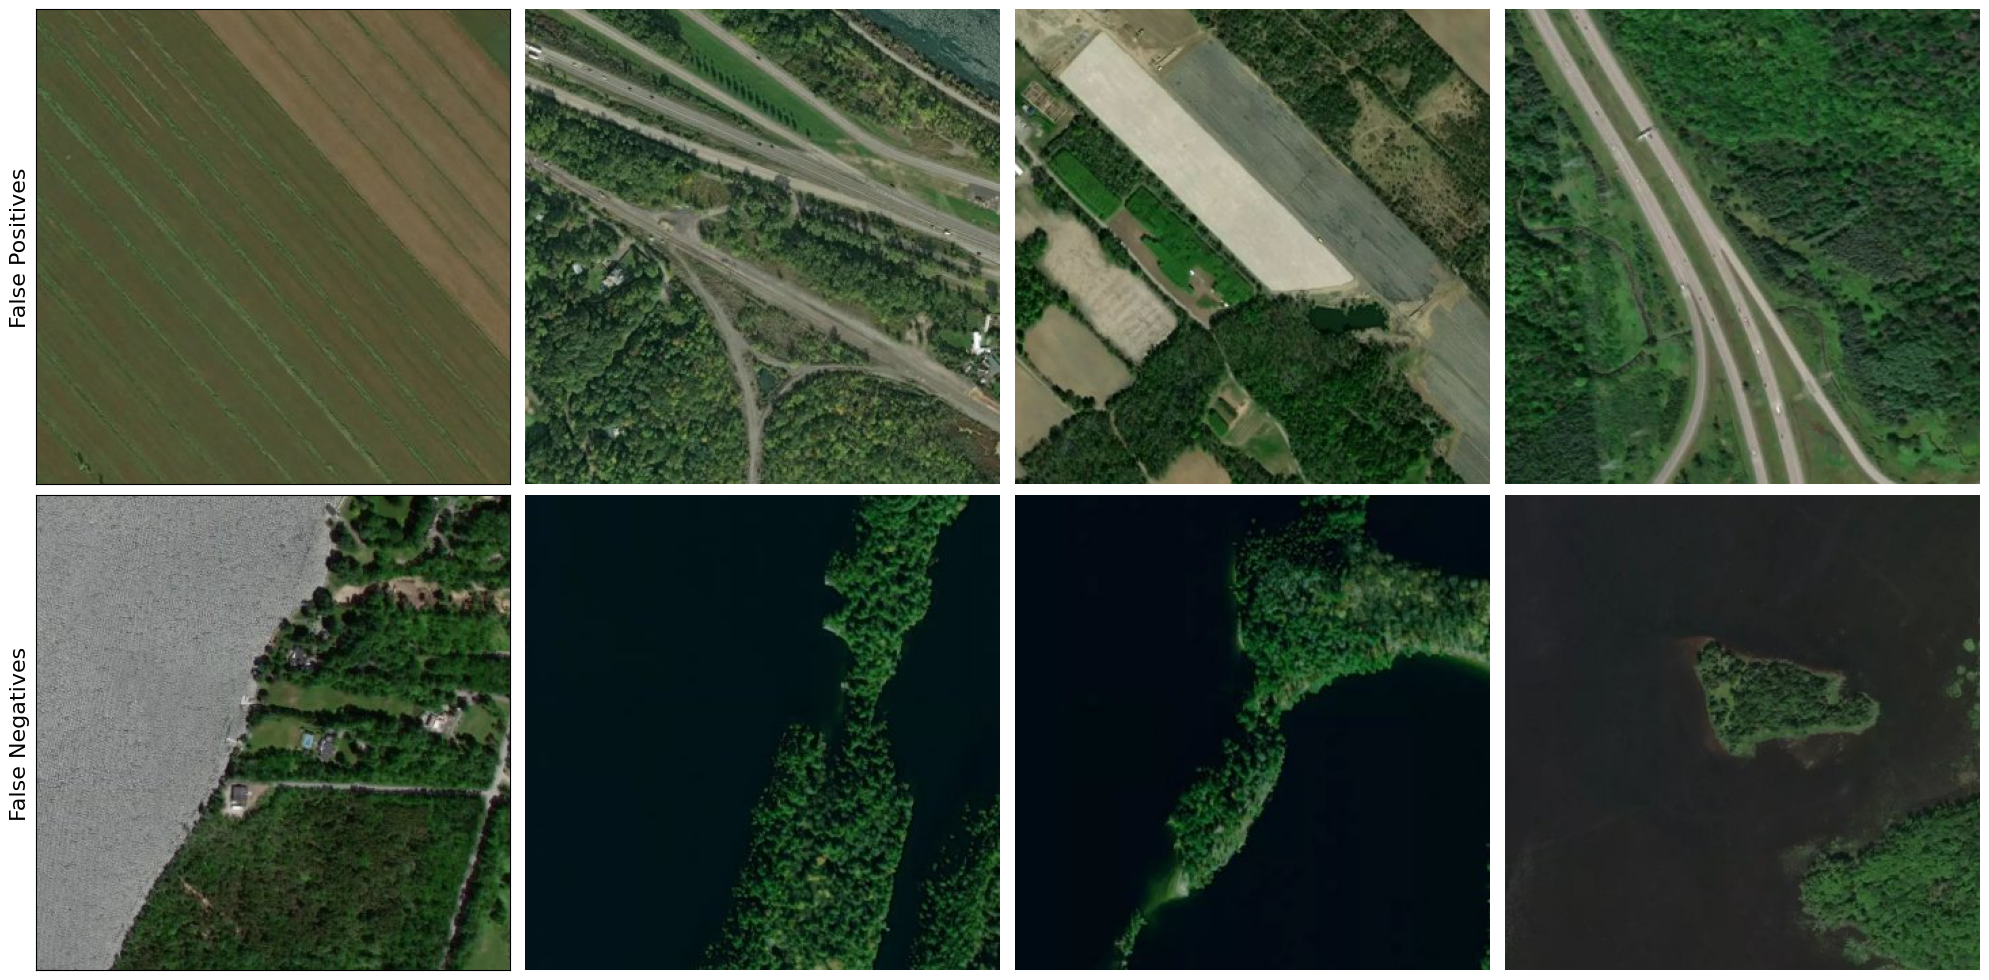
\includegraphics[width=\textwidth]{figures/errors3.png}
    \caption{Misclassified Samples. Top and bottom rows show false positives and false negatives respectively.}
  \end{subfigure}
  \caption{Error Analysis: (a) Confusion Matrix of the best model, (b) Misclassified samples.}
  \label{fig:error_analysis}
\end{figure}

We observe that most false negatives occur when the image has occlusions, such
as by clouds, or large patches of water or monochromatic fields. On the other
hand, it is not entirely clear why the model misclassifies some of the false
positives, but a visual inspection showed that these images contain a lot of
vegetation and are visually similar to wildfire images.

\section{Conclusion}

In this study, we evaluated various classification models with and without
pre-training to assess their performance in leveraging coordinate-based and
feature-based learning. Our findings demonstrate that the incorporation of
coordinate information significantly enhances classification performance across
all architectures.

Pre-training methods such as SimCLR, pseudo-labeling, and variational
autoencoders exhibit potential but do not consistently surpass the best fully
supervised models. Among them, pseudo-labeling provides notable improvements
for CNN-based models, while SimCLR achieves competitive performance with
ResNet50. However, latent representation learning approaches, including
$\beta$-VAE and VQ-VAE, yield lower accuracy, suggesting that their learned
representations may not be as effective as direct feature extraction from
supervised learning.

These results indicate that direct supervised learning with a well-structured
feature extractor, complemented by coordinate information, remains the most
effective approach for this classification task.

Future work could explore de-biasing the model to reduce errors on occluded
images and to decorrelate wildfires with vegetation and investigate additional
pre-training strategies to further enhance classification performance.

%Bibliography
\bibliographystyle{unsrt}
\bibliography{references}

\end{document}
